\documentclass[12pt,letterpaper]{article}

% ---------------------------------------------------------------------------
% Paquetes
% ---------------------------------------------------------------------------
\usepackage[utf8]{inputenc}
\usepackage[T1]{fontenc}
\usepackage[spanish,es-nodecimaldot,es-noshorthands]{babel}
\usepackage[margin=2.5cm]{geometry}
\usepackage{amsmath,amssymb}
\usepackage{graphicx}
\usepackage{float}
\usepackage{booktabs}
\usepackage{makecell}
\usepackage{caption}
\usepackage{siunitx}
\usepackage{listings}
\usepackage{xcolor}
\usepackage[hidelinks]{hyperref}

\graphicspath{{figuras/}}

\sisetup{
  output-decimal-marker = {.},
  group-digits = false,
  exponent-product = \times,
  per-mode = symbol
}

\captionsetup{font=small, labelfont=bf}
\renewcommand{\theadfont}{\small\bfseries}

\lstset{
  language=Python,
  basicstyle=\ttfamily\small,
  keywordstyle=\bfseries,
  commentstyle=\itshape\color{gray},
  numbers=none,
  frame=single,
  breaklines=true,
  columns=fullflexible,
  keepspaces=true,
  showstringspaces=false,
  literate={á}{{\'a}}1 {é}{{\'e}}1 {í}{{\'i}}1 {ó}{{\'o}}1 {ú}{{\'u}}1 {ñ}{{\~n}}1
}
\AtBeginDocument{\renewcommand{\lstlistingname}{Listado}}

% Operadores
\DeclareMathOperator{\atanh}{atanh}
\DeclareMathOperator{\acosh}{acosh}
\newcommand{\vt}{v_t}
\newcommand{\bs}{\mathbf{s}}
\newcommand{\bk}{\mathbf{k}}
\newcommand{\bff}{\mathbf{f}}

% ---------------------------------------------------------------------------
% Portada
% ---------------------------------------------------------------------------
\title{Caída libre con resistencia del aire\\[0.3em]
\large Proyecto final de Modelación y Simulación 2026\\
Opción 2: Simulación de un fenómeno dinámico}
\author{Víctor Pérez, Melisa Mendizabal, Renato Rojas}
\date{21 de noviembre de 2026}

\begin{document}

\maketitle

\begin{abstract}
Se simula la caída vertical de un cuerpo sometido a la gravedad y a la resistencia del aire, resolviendo numéricamente la ecuación de movimiento con dos métodos implementados desde cero: Euler explícito y Runge-Kutta de orden~4 (RK4). Se comparan tres modelos de arrastre (vacío, lineal y cuadrático) en dos escenarios: un paracaidista que salta desde \qty{4000}{m} y cuatro pelotas reales soltadas desde \qty{56}{m}, la altura aproximada de la Torre de Pisa. Todas las simulaciones se validan contra las soluciones analíticas de cada modelo. Los resultados muestran que la resistencia del aire reduce la rapidez de impacto del paracaidista de \qty{280}{m/s} a \qty{51}{m/s}, que la forma de la ley de arrastre cambia la transición hacia la velocidad terminal aun cuando esta es la misma, y que lo que determina la influencia del aire en una pelota es la relación entre su masa y su área, no la masa sola. El análisis de convergencia confirma los órdenes teóricos de ambos métodos (1.00 y 4.0) y muestra que, por debajo de cierto paso de tiempo, el error de RK4 queda dominado por el redondeo de punto flotante.
\end{abstract}

% ---------------------------------------------------------------------------
% Cuerpo del informe, dividido en archivos para trabajar en paralelo.
%   Parte 1 (secciones/parte1_teoria.tex): fenómeno, marco teórico, métodos y metodología.
%   Parte 2 (secciones/parte2_resultados.tex y secciones/apendices.tex): resultados,
%           conclusiones, limitaciones y apéndices.
% ---------------------------------------------------------------------------
% Parte 1: fenómeno, marco teórico, métodos y metodología.
% Se incluye desde informe.tex; no compilar este archivo solo.

% ===========================================================================
\section{Explicación del fenómeno}
% ===========================================================================

Un cuerpo que cae en el aire está sometido a dos fuerzas: su peso, que es constante, y la resistencia del aire (arrastre), que se opone al movimiento y crece con la rapidez. Al inicio de la caída el cuerpo se mueve despacio, el arrastre es pequeño y el cuerpo acelera casi como lo haría en el vacío. A medida que gana rapidez el arrastre aumenta, hasta que llega a igualar al peso. En ese momento la fuerza neta es cero, la aceleración desaparece y el cuerpo sigue cayendo a rapidez constante. Esa rapidez límite se llama \emph{velocidad terminal} y se denota $\vt$.

Este comportamiento tiene consecuencias prácticas importantes. Un paracaidista en caída libre no acelera indefinidamente, sino que se estabiliza alrededor de los \qty{180}{km/h}; una gota de lluvia llega al suelo a pocos metros por segundo en lugar de hacerlo a la rapidez que tendría tras caer cientos de metros en el vacío. También explica por qué el resultado del experimento atribuido a Galileo, en el que objetos de distinta masa caen al mismo tiempo, solo se cumple de forma aproximada en presencia de aire.

En este proyecto se estudia esta dinámica en una dimensión (solo movimiento vertical). Se comparan dos leyes de arrastre, una lineal y una cuadrática, junto con la caída en el vacío como referencia, en dos situaciones:
\begin{enumerate}
  \item un paracaidista en caída libre desde \qty{4000}{m};
  \item cuatro pelotas de distintos deportes soltadas desde \qty{56}{m}.
\end{enumerate}
Además, se valida la implementación numérica con un análisis de convergencia de los dos métodos de integración utilizados.

% ===========================================================================
\section{Marco teórico}
% ===========================================================================

\subsection{Ecuación de movimiento}

Se toma el eje $y$ positivo hacia arriba y se describe el estado del cuerpo con su altura $y$ y su velocidad $v$. Por la segunda ley de Newton, el movimiento queda descrito por el sistema de dos ecuaciones diferenciales ordinarias de primer orden
\begin{equation}
  \frac{dy}{dt} = v, \qquad \frac{dv}{dt} = -g + \frac{F_d(v)}{m},
  \label{eq:movimiento}
\end{equation}
donde $m$ es la masa del cuerpo, $g$ la aceleración de la gravedad y $F_d(v)$ la fuerza de arrastre. Como el cuerpo cae, $v<0$ durante todo el movimiento.

\subsection{Modelos de arrastre}

Se consideran tres modelos para $F_d$, resumidos en el Cuadro~\ref{tab:modelos}. En cada caso, la velocidad terminal se obtiene al igualar el arrastre con el peso, es decir, al imponer $\dot v = 0$.

\begin{table}[H]
  \centering
  \caption{Modelos de arrastre considerados.}
  \label{tab:modelos}
  \renewcommand{\arraystretch}{1.6}
  \begin{tabular}{@{}llll@{}}
    \toprule
    Modelo & Fuerza $F_d(v)$ & Ecuación para $v$ & Velocidad terminal \\
    \midrule
    Vacío & $0$ & $\dot v = -g$ & no existe \\
    Lineal (Stokes) & $-b\,v$ & $\dot v = -g - \dfrac{b}{m}\,v$ & $\vt = \dfrac{mg}{b}$ \\
    Cuadrático & $-k\,v\lvert v\rvert$ & $\dot v = -g - \dfrac{k}{m}\,v\lvert v\rvert$ & $\vt = \sqrt{\dfrac{mg}{k}}$ \\
    \bottomrule
  \end{tabular}
\end{table}

En el modelo cuadrático, la constante de arrastre es
\begin{equation}
  k = \tfrac12 \rho\, C_d\, A,
  \qquad\text{de modo que}\qquad
  \vt = \sqrt{\frac{2mg}{\rho\, C_d\, A}},
  \label{eq:k}
\end{equation}
donde $\rho$ es la densidad del aire, $C_d$ el coeficiente de arrastre y $A$ el área frontal del cuerpo. Se usa $v\lvert v\rvert$ en lugar de $v^2$ para que la fuerza siempre se oponga al movimiento, sin importar el signo de $v$.

\subsection{Validez de cada modelo: número de Reynolds}

El modelo adecuado depende del régimen del flujo alrededor del cuerpo, que se caracteriza con el número de Reynolds
\begin{equation}
  Re = \frac{\rho\, \lvert v\rvert\, L}{\mu},
  \label{eq:reynolds}
\end{equation}
donde $L$ es una longitud característica (el diámetro, en el caso de una esfera) y $\mu$ la viscosidad dinámica del aire. El arrastre lineal solo es válido en el régimen de Stokes, $Re \lesssim 1$, que corresponde a partículas microscópicas como polvo o gotas de niebla. Para objetos macroscópicos en aire, en el rango $10^3 < Re < 2\times10^5$, el coeficiente $C_d$ de una esfera es aproximadamente constante (cercano a 0.47) y el arrastre es cuadrático~\cite{white}.

Para dimensionar esto, la rapidez a la que $Re = 1$ es $v = \mu/(\rho L)$. Para una pelota de ping-pong esa rapidez es de \qty{0.00037}{m/s} y para una bola de boliche de \qty{0.000068}{m/s}. Cualquier caída real de estos objetos ocurre a rapideces varios órdenes de magnitud mayores, así que el modelo lineal no les aplica. En este proyecto el modelo lineal se usa como punto de comparación y para validar los métodos numéricos, ya que tiene una solución exacta sencilla.

\subsection{Soluciones analíticas}
\label{sec:analiticas}

Los tres modelos tienen solución cerrada, lo que permite medir con exactitud el error de los métodos numéricos. Se denota $h_0$ la altura inicial y $v_0 \le 0$ la velocidad inicial; en todos los escenarios de este trabajo $v_0 = 0$.

\paragraph{Vacío.}
\begin{equation}
  v(t) = v_0 - g t, \qquad y(t) = h_0 + v_0 t - \tfrac12 g t^2 .
\end{equation}
Desde el reposo, el tiempo de caída es $t = \sqrt{2h_0/g}$ y la rapidez de impacto es $\sqrt{2gh_0}$.

\paragraph{Arrastre lineal.} Con $\tau = m/b$,
\begin{align}
  v(t) &= -\vt + (v_0 + \vt)\, e^{-t/\tau}, \\
  y(t) &= h_0 - \vt t + \tau\,(v_0 + \vt)\left(1 - e^{-t/\tau}\right).
\end{align}
La rapidez se acerca a $\vt$ de forma exponencial. Desde el reposo, el tiempo para alcanzar el \qty{95}{\percent} de $\vt$ es $t_{95} = \tau \ln 20$.

\paragraph{Arrastre cuadrático.} Para $-\vt < v_0 \le 0$, con $\tau_0 = \atanh(\lvert v_0\rvert/\vt)$~\cite{taylor},
\begin{align}
  v(t) &= -\vt \tanh\!\left(\frac{g t}{\vt} + \tau_0\right), \\
  y(t) &= h_0 - \frac{\vt^2}{g}\,
          \ln\frac{\cosh\!\left(\frac{g t}{\vt} + \tau_0\right)}{\cosh \tau_0}.
\end{align}
Desde el reposo, el tiempo para alcanzar el \qty{95}{\percent} de $\vt$ y el tiempo de caída hasta el suelo son
\begin{equation}
  t_{95} = \frac{\vt}{g}\,\atanh(0.95),
  \qquad
  t_{\text{imp}} = \frac{\vt}{g}\,\acosh\!\left(e^{g h_0/\vt^2}\right).
\end{equation}

En caídas largas, $\cosh x$ excede el rango de los números de punto flotante. Por eso, en la implementación se evalúa $\ln\cosh x$ mediante la identidad equivalente y numéricamente estable
\begin{equation}
  \ln\cosh x = \lvert x\rvert + \ln\!\left(1 + e^{-2\lvert x\rvert}\right) - \ln 2 .
\end{equation}

% ===========================================================================
\section{Métodos de simulación}
% ===========================================================================

El sistema~\eqref{eq:movimiento} se escribe en forma vectorial con el estado $\bs = (y, v)$ y $\bff(\bs) = (v,\ a(v))$, donde $a(v) = -g + F_d(v)/m$. Para integrarlo se implementaron dos métodos de paso fijo, sin recurrir a bibliotecas como \texttt{scipy}~\cite{burden}.

\subsection{Euler explícito}

Es el método más simple: avanza el estado usando la derivada evaluada al inicio del paso,
\begin{equation}
  \bs_{n+1} = \bs_n + \Delta t\, \bff(\bs_n).
\end{equation}
Su error global es $O(\Delta t)$, es decir, es de orden~1.

\subsection{Runge-Kutta de orden 4}

RK4 combina cuatro evaluaciones de la derivada dentro de cada paso:
\begin{gather}
  \bk_1 = \bff(\bs_n), \quad
  \bk_2 = \bff\!\left(\bs_n + \tfrac{\Delta t}{2}\bk_1\right), \quad
  \bk_3 = \bff\!\left(\bs_n + \tfrac{\Delta t}{2}\bk_2\right), \quad
  \bk_4 = \bff(\bs_n + \Delta t\,\bk_3), \\
  \bs_{n+1} = \bs_n + \frac{\Delta t}{6}\left(\bk_1 + 2\bk_2 + 2\bk_3 + \bk_4\right).
\end{gather}
Su error global es $O(\Delta t^4)$. En la práctica, al dividir el paso entre 10 el error de Euler disminuye 10 veces y el de RK4 disminuye \num{10000} veces. A cambio, RK4 requiere 4 evaluaciones de $\bff$ por paso en lugar de una; medido en nuestra implementación, cada paso de RK4 tarda entre 4.5 y 5 veces más que uno de Euler.

\subsection{Detección del impacto con el suelo}

La integración avanza hasta el primer paso en el que $y \le 0$. Como el impacto ocurre, en general, entre dos pasos, su instante y su velocidad se estiman por interpolación lineal entre el último punto con $y > 0$ y el primero con $y \le 0$:
\begin{equation}
  s = \frac{y_n}{y_n - y_{n+1}}, \qquad
  t_{\text{imp}} = t_n + s\,\Delta t, \qquad
  v_{\text{imp}} = v_n + s\,(v_{n+1} - v_n).
\end{equation}

\subsection{Implementación}

El simulador está escrito en Python, usando únicamente \texttt{numpy} para los arreglos y \texttt{matplotlib} para las figuras. El código se organiza en el paquete \texttt{freefall}:
\begin{itemize}
  \item \texttt{models.py}: cuerpos (masa, $C_d$, área, longitud característica) y modelos de arrastre;
  \item \texttt{analytic.py}: soluciones exactas de la Sección~\ref{sec:analiticas};
  \item \texttt{solvers.py}: pasos de Euler y RK4 e integración con detección del impacto;
  \item \texttt{scenarios.py}: parámetros de los escenarios y cálculo de métricas;
  \item \texttt{convergence.py}: errores contra la solución analítica y orden observado;
  \item \texttt{plots.py}, \texttt{report.py} y \texttt{\_\_main\_\_.py}: figuras, tablas e interfaz de línea de comandos.
\end{itemize}
Cada modelo de arrastre es una clase que implementa la aceleración $a(v)$ y la velocidad terminal, de modo que los integradores son independientes del modelo. El Listado~\ref{lst:solvers} muestra el núcleo de los integradores.

\begin{lstlisting}[caption={Pasos de Euler y RK4 y detección del impacto (\texttt{solvers.py}).}, label={lst:solvers}]
def euler_step(f, state, dt):
    return state + dt * f(state)

def rk4_step(f, state, dt):
    k1 = f(state)
    k2 = f(state + 0.5 * dt * k1)
    k3 = f(state + 0.5 * dt * k2)
    k4 = f(state + dt * k3)
    return state + dt / 6 * (k1 + 2 * k2 + 2 * k3 + k4)

# Dentro del ciclo de integración:
new = step(f, states[-1], dt)
if stop_at_ground and new[0] <= 0:
    old = states[-1]
    s = old[0] / (old[0] - new[0])
    impact_time = times[-1] + s * dt
    impact_velocity = old[1] + s * (new[1] - old[1])
\end{lstlisting}

% ===========================================================================
\section{Metodología}
% ===========================================================================

\subsection{Parámetros generales}

El Cuadro~\ref{tab:constantes} resume las constantes físicas y numéricas comunes a todos los escenarios. Salvo que se indique lo contrario, todas las simulaciones usan RK4 con $\Delta t = \qty{0.01}{s}$ y parten del reposo.

\begin{table}[H]
  \centering
  \caption{Constantes usadas en todos los escenarios.}
  \label{tab:constantes}
  \begin{tabular}{@{}ll@{}}
    \toprule
    Constante & Valor \\
    \midrule
    Gravedad $g$ & \qty{9.81}{m/s^2} \\
    Densidad del aire $\rho$ & \qty{1.225}{kg/m^3} (nivel del mar, \qty{15}{\degreeCelsius}) \\
    Viscosidad dinámica del aire $\mu$ & \qty{1.81e-5}{\pascal\second} \\
    Paso de tiempo por defecto $\Delta t$ & \qty{0.01}{s} \\
    Método por defecto & RK4 \\
    \bottomrule
  \end{tabular}
\end{table}

\subsection{Escenario 1: paracaidista}

Se simula un salto desde \qty{4000}{m} en posición de vientre abajo, sin abrir el paracaídas, desde el reposo hasta el suelo. Los parámetros se muestran en el Cuadro~\ref{tab:paracaidista-param}. Se comparan los tres modelos: vacío, lineal y cuadrático.

\begin{table}[H]
  \centering
  \caption{Parámetros del paracaidista.}
  \label{tab:paracaidista-param}
  \begin{tabular}{@{}ll@{}}
    \toprule
    Parámetro & Valor \\
    \midrule
    Masa $m$ & \qty{80}{kg} \\
    Coeficiente de arrastre $C_d$ & 1.0 \\
    Área frontal $A$ & \qty{0.5}{m^2} \\
    Longitud característica $L$ (para $Re$) & \qty{1.8}{m} \\
    $k = \tfrac12\rho C_d A$ & \qty{0.30625}{kg/m} \\
    Velocidad terminal (cuadrático) & \qty{50.62}{m/s} (\qty{182}{km/h}) \\
    $b$ del modelo lineal & \qty{15.503}{kg/s} \\
    $\tau = m/b = \vt/g$ & \qty{5.160}{s} \\
    $Re$ a velocidad terminal & \num{6.2e6} \\
    \bottomrule
  \end{tabular}
\end{table}

Una decisión de diseño importante es la elección de $b$. Su valor no se tomó de la física del problema (el modelo lineal no aplica a un paracaidista, cuyo $Re$ es del orden de $10^6$), sino que se \emph{calibró para que la velocidad terminal fuera la misma que en el modelo cuadrático}: $b = mg/\vt$. De esta forma las curvas de ambos modelos terminan en el mismo valor y la comparación aísla únicamente la diferencia de forma entre una ley de arrastre lineal y una cuadrática. Con esta calibración, además, la escala de tiempo $m/b$ del modelo lineal coincide con $\vt/g$, la escala natural del modelo cuadrático (\qty{5.16}{s} en ambos casos).

\subsection{Escenario 2: comparación de pelotas}

Se sueltan desde el reposo cuatro pelotas reales a \qty{56}{m} de altura, la altura aproximada de la Torre de Pisa, en referencia al experimento atribuido a Galileo. Se usa el modelo cuadrático con $C_d = 0.47$ (esfera lisa) y la caída en el vacío como referencia. Las masas y los radios corresponden a los valores reglamentarios de cada deporte (la bola de boliche es de 16~lb). El Cuadro~\ref{tab:pelotas-param} muestra los parámetros y la velocidad terminal resultante.

\begin{table}[H]
  \centering
  \small
  \caption{Parámetros de las pelotas ($C_d = 0.47$).}
  \label{tab:pelotas-param}
  \begin{tabular}{@{}lrrrrrr@{}}
    \toprule
    Pelota & \thead{Masa\\(kg)} & \thead{Radio\\(m)} & \thead{Diámetro\\(m)} & \thead{Área $A$\\(m$^2$)} & \thead{$k$\\(kg/m)} & \thead{$\vt$\\(m/s)} \\
    \midrule
    Ping-pong & 0.0027 & 0.020  & 0.040  & 0.001257 & 0.000362 & 8.56 \\
    Tenis     & 0.058  & 0.0335 & 0.067  & 0.003526 & 0.001015 & 23.68 \\
    Béisbol   & 0.145  & 0.0366 & 0.0732 & 0.004208 & 0.001211 & 34.27 \\
    Boliche   & 7.26   & 0.108  & 0.216  & 0.036644 & 0.010549 & 82.17 \\
    \bottomrule
  \end{tabular}
\end{table}

La pregunta que busca responder este escenario es qué tanto importa el aire en una caída corta, dependiendo de la relación entre la masa y el área de cada pelota.

\subsection{Escenario 3: validación y convergencia}
\label{sec:diseno-convergencia}

Para validar los métodos y medir su orden de convergencia se diseñó el siguiente experimento:
\begin{itemize}
  \item \textbf{Caso de prueba:} el paracaidista del Escenario~1 con los modelos lineal y cuadrático, integrado con Euler y con RK4.
  \item \textbf{Intervalo:} se integra en $[0, 20]$~s \emph{sin detener la simulación en el suelo}. Así el error medido corresponde solo al integrador y no se mezcla con el de la interpolación del impacto.
  \item \textbf{Pasos de tiempo:} 13 valores de $\Delta t$: 1, 0.5, 0.25, 0.1, 0.05, 0.025, 0.01, 0.005, 0.0025, 0.001, 0.0005, 0.00025 y 0.0001~s.
  \item \textbf{Métrica:} para cada paso se mide el error absoluto máximo en $y$ y en $v$ contra la solución analítica.
  \item \textbf{Orden observado:} es la pendiente de un ajuste lineal de $\log(\text{error})$ contra $\log(\Delta t)$. Se descartan el paso de \qty{1}{s} y los puntos con error menor a $10^{-9}$, donde domina el error de redondeo.
  \item \textbf{Orden local:} también se calcula el orden entre pasos consecutivos,
  $p_i = \dfrac{\log(e_{i-1}/e_i)}{\log(\Delta t_{i-1}/\Delta t_i)}$.
\end{itemize}
Adicionalmente, se repiten los escenarios 1 y 2 con Euler para medir el efecto del método en los resultados, y se integra el modelo cuadrático con un paso grande ($\Delta t = \qty{2}{s}$) para ilustrar visualmente la diferencia entre ambos métodos.


% Parte 2: resultados, conclusiones y limitaciones.
% Se incluye desde informe.tex; no compilar este archivo solo.

% ===========================================================================
\section{Resultados y visualizaciones}
% ===========================================================================

\subsection{Escenario 1: paracaidista}

El Cuadro~\ref{tab:paracaidista-res} resume las métricas de cada modelo y la Figura~\ref{fig:paracaidista} muestra la evolución de la altura, la rapidez y la aceleración. $t_{95}$ es el tiempo necesario para alcanzar el \qty{95}{\percent} de la velocidad terminal y $d_{95}$ la distancia recorrida hasta ese instante.

\begin{table}[H]
  \centering
  \small
  \caption{Resultados del paracaidista (RK4, $\Delta t = \qty{0.01}{s}$).}
  \label{tab:paracaidista-res}
  \begin{tabular}{@{}lrrrrr@{}}
    \toprule
    Modelo & \thead{$\vt$\\(m/s)} & \thead{$t_{95}$\\(s)} & \thead{$d_{95}$\\(m)} & \thead{Tiempo de\\caída (s)} & \thead{Rapidez de\\impacto (m/s)} \\
    \midrule
    Vacío      & ---    & ---    & ---   & 28.557 & 280.143 \\
    Lineal     & 50.622 & 15.459 & 534.4 & 84.177 & 50.622 \\
    Cuadrático & 50.622 & 9.452  & 304.1 & 82.593 & 50.622 \\
    \bottomrule
  \end{tabular}
\end{table}

\begin{figure}[H]
  \centering
  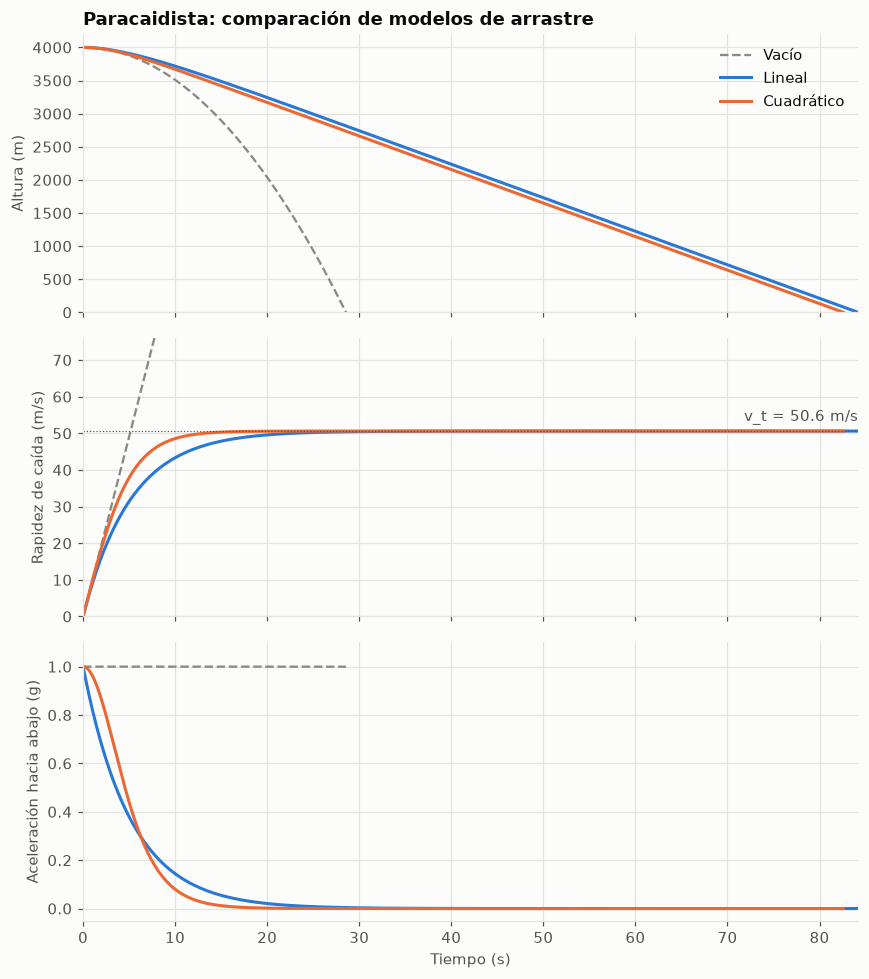
\includegraphics[width=0.82\textwidth]{paracaidista_modelos.png}
  \caption{Paracaidista: altura, rapidez de caída $\lvert v\rvert$ y aceleración hacia abajo (en unidades de $g$) para los tres modelos. En la aceleración, 1 corresponde a caída libre sin aire y 0 al régimen terminal. La línea punteada horizontal marca $\vt = \qty{50.6}{m/s}$.}
  \label{fig:paracaidista}
\end{figure}

\paragraph{Validación.} Los valores simulados coinciden con las fórmulas de la Sección~\ref{sec:analiticas}:
\begin{itemize}
  \item Vacío: $\sqrt{2\cdot 4000/9.81} = \qty{28.5569}{s}$ y $\sqrt{2\cdot 9.81\cdot 4000} = \qty{280.143}{m/s}$. Simulado: \qty{28.5569}{s} y \qty{280.143}{m/s}.
  \item Lineal: $t_{95} = 5.160\ln 20 = \qty{15.459}{s}$. Simulado: \qty{15.459}{s}.
  \item Cuadrático: $t_{95} = 5.160\,\atanh(0.95) = \qty{9.452}{s}$ y $t_{\text{imp}} = \qty{82.5935}{s}$. Simulado: \qty{9.452}{s} y \qty{82.5935}{s}.
\end{itemize}

\paragraph{Discusión.}
Aunque ambos modelos tienen la misma velocidad terminal, el cuadrático llega al \qty{95}{\percent} de $\vt$ en \qty{9.5}{s} y el lineal en \qty{15.5}{s}, es decir, un \qty{64}{\percent} más tarde. La razón está en la forma de cada ley: el arrastre cuadrático es débil a baja rapidez, por lo que al principio el cuerpo acelera casi como en el vacío, pero crece muy rápido al acercarse a $\vt$, lo que produce una transición más abrupta. El arrastre lineal, en cambio, frena desde el primer instante y se aproxima a $\vt$ más lentamente. Esto se observa con claridad en el panel inferior de la Figura~\ref{fig:paracaidista}: la aceleración del modelo lineal disminuye de inmediato, mientras que la del cuadrático se mantiene cerca de $1\,g$ durante los primeros segundos y luego cae bruscamente.

Como el paracaidista pasa unos \qty{70}{s} en régimen terminal, los tiempos totales de caída de ambos modelos difieren solo en \qty{1.6}{s} (\qty{2}{\percent}); la diferencia entre modelos se concentra en los primeros 15 a \qty{20}{s}. En régimen terminal el paracaidista desciende unos \qty{50}{m} cada segundo, por eso la curva de altura es casi una recta durante la mayor parte del salto.

Sin aire, el paracaidista llegaría al suelo en \qty{28.6}{s} a \qty{280}{m/s} (\qty{1008}{km/h}), una rapidez 5.5 veces mayor que con aire. La resistencia del aire, por tanto, no es un detalle en este problema: determina por completo el resultado.

\subsection{Escenario 2: pelotas}

El Cuadro~\ref{tab:pelotas-res} resume los resultados de la caída de las cuatro pelotas. La Figura~\ref{fig:pelotas-tray} muestra las trayectorias y la Figura~\ref{fig:pelotas-resumen} condensa el escenario en dos indicadores.

\begin{table}[H]
  \centering
  \small
  \caption{Resultados de las pelotas desde \qty{56}{m} (RK4, $\Delta t = \qty{0.01}{s}$).}
  \label{tab:pelotas-res}
  \begin{tabular}{@{}lrrrrrr@{}}
    \toprule
    Pelota & \thead{$\vt$\\(m/s)} & \thead{Tiempo de\\caída (s)} & \thead{Retraso vs.\\vacío (s)} & \thead{Rapidez de\\impacto (m/s)} & \thead{\% de $\vt$\\al impactar} & \thead{$Re$ al\\impactar} \\
    \midrule
    Ping-pong & 8.557  & 7.149 & 3.770 & 8.557  & 100.0 & \num{23165} \\
    Tenis     & 23.677 & 3.948 & 0.569 & 21.946 & 92.7  & \num{99515} \\
    Béisbol   & 34.266 & 3.647 & 0.269 & 26.712 & 78.0  & \num{132336} \\
    Boliche   & 82.168 & 3.425 & 0.046 & 31.843 & 38.8  & \num{465506} \\
    Vacío     & ---    & 3.379 & 0     & 33.147 & ---   & --- \\
    \bottomrule
  \end{tabular}
\end{table}

\paragraph{Validación.} En el vacío, $\sqrt{2\cdot 56/9.81} = \qty{3.3789}{s}$ y $\sqrt{2\cdot 9.81\cdot 56} = \qty{33.147}{m/s}$. Simulado: \qty{3.3789}{s} y \qty{33.147}{m/s}.

\begin{figure}[H]
  \centering
  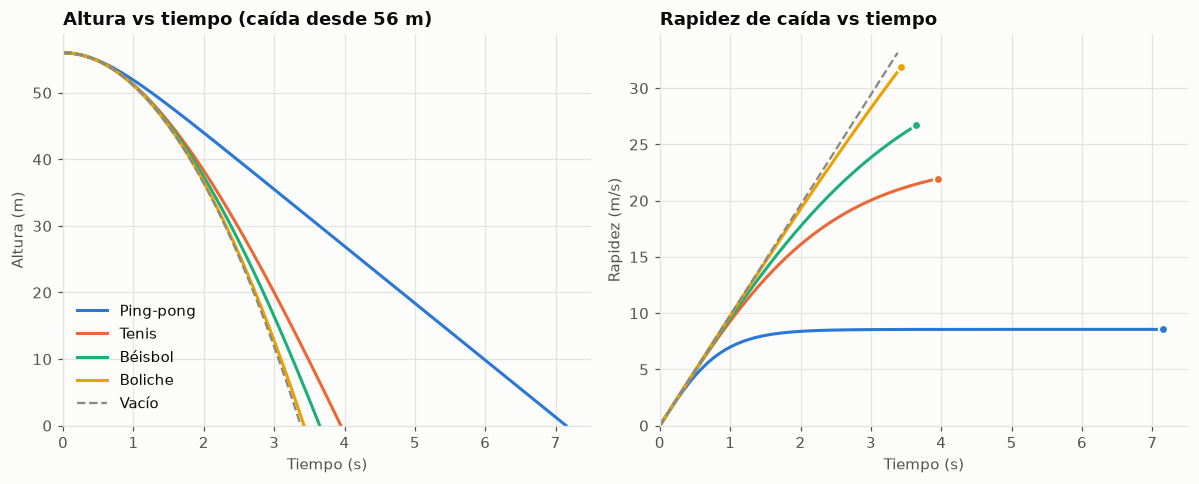
\includegraphics[width=\textwidth]{pelotas_trayectorias.png}
  \caption{Altura y rapidez de caída contra el tiempo para las cuatro pelotas y la caída en el vacío. El punto al final de cada curva de rapidez marca el impacto con el suelo.}
  \label{fig:pelotas-tray}
\end{figure}

\begin{figure}[H]
  \centering
  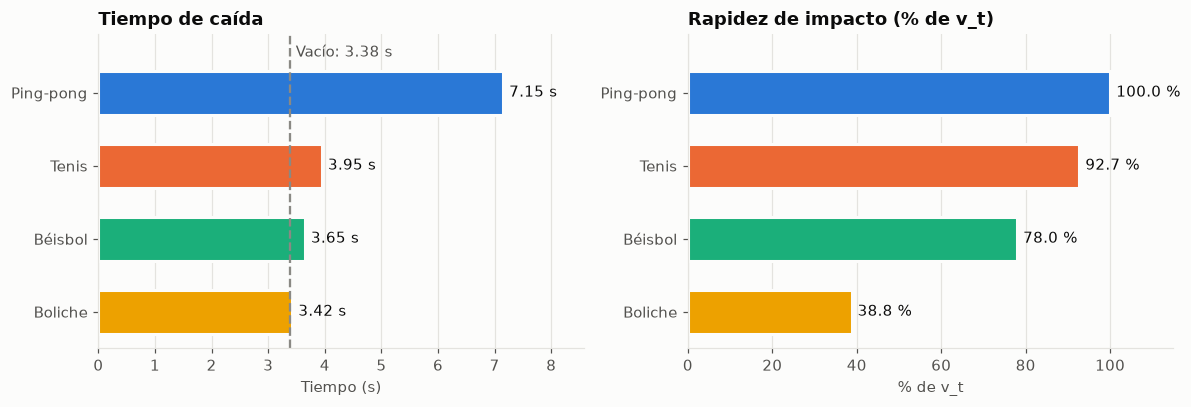
\includegraphics[width=\textwidth]{pelotas_resumen.png}
  \caption{Izquierda: tiempo de caída de cada pelota; la línea discontinua indica el tiempo en el vacío. Derecha: rapidez de impacto como porcentaje de la velocidad terminal de cada pelota.}
  \label{fig:pelotas-resumen}
\end{figure}

\paragraph{Discusión.}
Lo que determina la influencia del aire no es la masa por sí sola, sino la relación $m/k$, es decir, la masa frente al área. Como $\vt = \sqrt{mg/k}$, una pelota pesada y compacta tiene una velocidad terminal alta y en una caída de \qty{56}{m} apenas nota el aire.

\begin{itemize}
  \item La bola de boliche llega solo \qty{0.046}{s} después que en el vacío (\qty{1.4}{\percent} más tarde). A simple vista caería ``como en el vacío'', lo que es coherente con la observación atribuida a Galileo. Al impactar apenas ha alcanzado el \qty{38.8}{\percent} de su velocidad terminal.
  \item La pelota de ping-pong alcanza su velocidad terminal (\qty{8.56}{m/s}) en menos de \qty{2}{s} y recorre el resto de la altura a rapidez constante: tarda \qty{7.15}{s}, más del doble que en el vacío.
  \item Las pelotas de tenis y de béisbol son casos intermedios: se separan claramente de la curva del vacío en la segunda mitad de la caída.
\end{itemize}

En cuanto al experimento de Galileo, en el vacío las cuatro pelotas caen exactamente igual. Con aire, la bola de boliche y la pelota de béisbol llegan al suelo con \qty{0.22}{s} de diferencia; cuando la bola de boliche toca el suelo, la de béisbol todavía está a unos \qty{6}{m} de altura.

Todos los números de Reynolds son mucho mayores que 1, lo que justifica el uso del modelo cuadrático. Las pelotas de ping-pong, tenis y béisbol ($Re$ entre \num{2e4} y \num{1.3e5}) están en el rango en que el $C_d$ de una esfera es aproximadamente constante. La bola de boliche ($Re \approx \num{4.7e5}$) ya se encuentra en la zona de la \emph{crisis de arrastre}, que para esferas lisas comienza alrededor de $Re \approx \num{2e5}$ a \num{3e5} y en la que $C_d$ puede disminuir bruscamente~\cite{white}. Sin embargo, como el aire solo modifica su tiempo de caída en un \qty{1.4}{\percent}, esto no altera las conclusiones.

\subsection{Escenario 3: convergencia y comparación de métodos}

\subsubsection{Orden de convergencia observado}

La Figura~\ref{fig:convergencia} muestra el error máximo contra el paso de tiempo en escala log-log y el Cuadro~\ref{tab:ordenes} los órdenes obtenidos con el ajuste descrito en la Sección~\ref{sec:diseno-convergencia}. Los órdenes medidos coinciden con los teóricos con un margen de \qty{1}{\percent}, lo que valida que ambos métodos están correctamente implementados. Las tablas completas de errores, con el orden local entre pasos consecutivos, se encuentran en el Apéndice~\ref{app:tablas}.

\begin{table}[H]
  \centering
  \caption{Orden de convergencia teórico y observado.}
  \label{tab:ordenes}
  \begin{tabular}{@{}llccc@{}}
    \toprule
    Modelo & Método & \thead{Orden\\teórico} & \thead{Orden observado\\en $y$} & \thead{Orden observado\\en $v$} \\
    \midrule
    Lineal     & Euler & 1 & 1.003 & 1.003 \\
    Lineal     & RK4   & 4 & 4.031 & 4.031 \\
    Cuadrático & Euler & 1 & 1.004 & 1.003 \\
    Cuadrático & RK4   & 4 & 3.996 & 4.037 \\
    \bottomrule
  \end{tabular}
\end{table}

\begin{figure}[H]
  \centering
  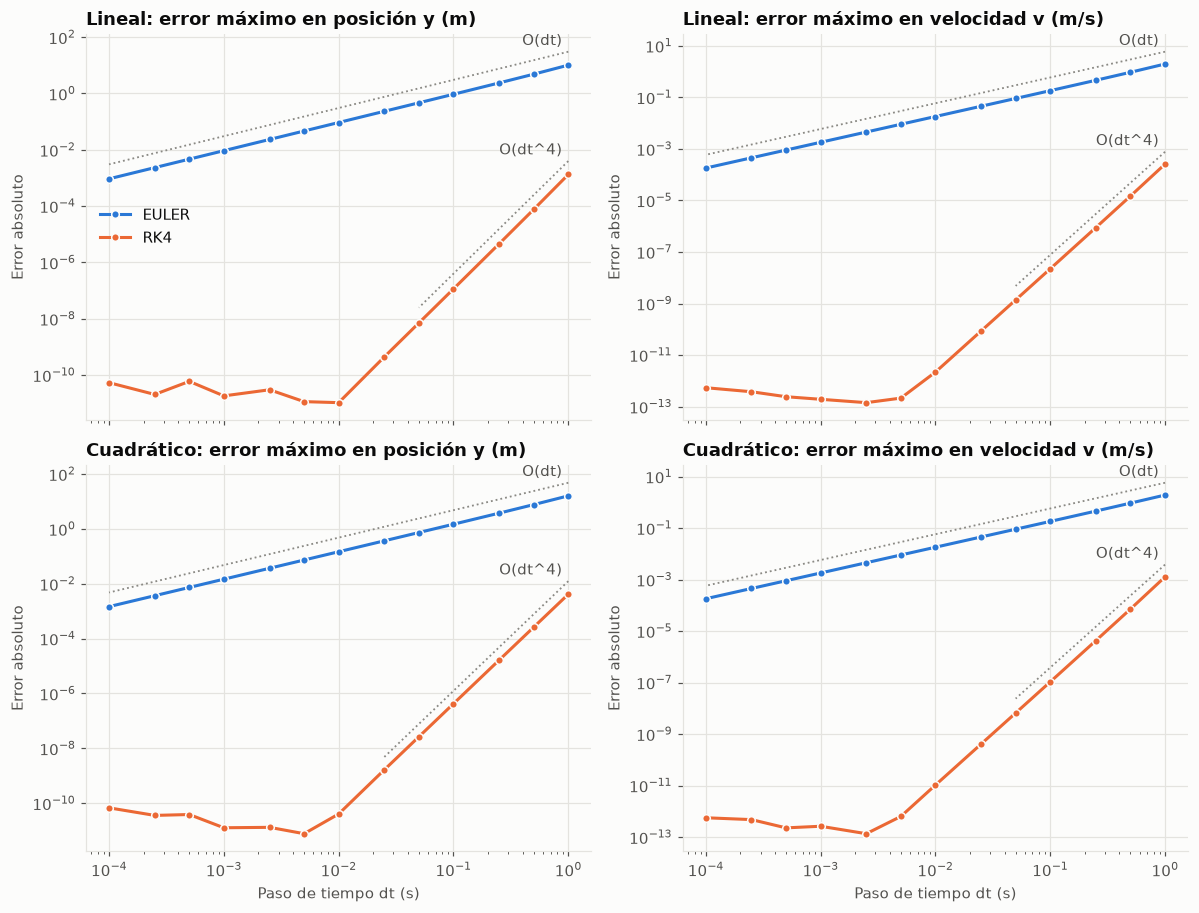
\includegraphics[width=\textwidth]{convergencia.png}
  \caption{Error absoluto máximo en $y$ y en $v$ contra el paso de tiempo $\Delta t$, para los modelos lineal y cuadrático en el intervalo $[0, 20]$~s. Las rectas punteadas son referencias de pendiente 1 y 4.}
  \label{fig:convergencia}
\end{figure}

\subsubsection{Errores y piso de redondeo}

El Cuadro~\ref{tab:errores} muestra una selección de los errores máximos para el modelo cuadrático.

\begin{table}[H]
  \centering
  \caption{Errores máximos seleccionados (modelo cuadrático, intervalo de \qty{20}{s}).}
  \label{tab:errores}
  \begin{tabular}{@{}lllll@{}}
    \toprule
    & \multicolumn{2}{c}{Euler} & \multicolumn{2}{c}{RK4} \\
    \cmidrule(lr){2-3} \cmidrule(l){4-5}
    $\Delta t$ (s) & Error en $y$ (m) & Error en $v$ (m/s) & Error en $y$ (m) & Error en $v$ (m/s) \\
    \midrule
    1      & 16.0   & 1.92    & \num{4.2e-3}  & \num{1.3e-3} \\
    0.1    & 1.48   & 0.182   & \num{4.2e-7}  & \num{1.1e-7} \\
    0.01   & 0.147  & 0.0181  & \num{4.0e-11} & \num{1.0e-11} \\
    0.001  & 0.0147 & 0.0018  & \num{1.3e-11} & \num{2.6e-13} \\
    0.0001 & 0.0015 & 0.00018 & \num{6.8e-11} & \num{5.6e-13} \\
    \bottomrule
  \end{tabular}
\end{table}

De estos resultados se destacan tres observaciones:
\begin{itemize}
  \item RK4 con $\Delta t = \qty{1}{s}$ es más preciso que Euler con $\Delta t = \qty{0.0001}{s}$, aun cuando este último realiza \num{10000} veces más pasos.
  \item \textbf{Piso de redondeo.} Por debajo de $\Delta t \approx \qty{0.01}{s}$ el error de RK4 deja de disminuir y se estanca entre $10^{-13}$ y $10^{-10}$; incluso aumenta ligeramente. En ese punto el error del método ya es menor que el error de redondeo de la aritmética de doble precisión (unos 16 dígitos significativos), que se acumula con el número de pasos. Reducir más el paso no mejora el resultado y solo aumenta el costo de cómputo.
  \item El error de Euler disminuye linealmente en todo el rango estudiado, porque en ningún momento llega al piso de redondeo.
\end{itemize}

\subsubsection{Efecto del método en los escenarios}

El Cuadro~\ref{tab:metodo-escenarios} compara los tiempos de caída obtenidos con cada método usando el paso por defecto. Con $\Delta t = \qty{0.01}{s}$, Euler ya produce resultados útiles, con errores del orden de milisegundos, mientras que RK4 coincide con la solución exacta en todos los dígitos mostrados.

\begin{table}[H]
  \centering
  \caption{Tiempo de caída con Euler y con RK4 ($\Delta t = \qty{0.01}{s}$).}
  \label{tab:metodo-escenarios}
  \begin{tabular}{@{}lrrr@{}}
    \toprule
    Caso & \thead{Euler\\(s)} & \thead{RK4\\(s)} & \thead{Diferencia\\(s)} \\
    \midrule
    Paracaidista, vacío      & 28.5619 & 28.5569 & 0.005 \\
    Paracaidista, cuadrático & 82.5954 & 82.5935 & 0.002 \\
    Ping-pong                & 7.1511  & 7.1491  & 0.002 \\
    Boliche                  & 3.4296  & 3.4249  & 0.005 \\
    Pelotas, vacío           & 3.3839  & 3.3789  & 0.005 \\
    \bottomrule
  \end{tabular}
\end{table}

\subsubsection{Paso de tiempo grande}

Para hacer visible la diferencia entre los métodos se integró el modelo cuadrático del paracaidista con $\Delta t = \qty{2}{s}$ (Figura~\ref{fig:dt-grande}). Euler llega a equivocarse en \qty{4.2}{m/s} a los \qty{6}{s}, en plena transición hacia $\vt$, y sobreestima la rapidez: al usar la aceleración del inicio de cada paso durante todo el paso, ``cree'' que el cuerpo acelera más de lo que realmente lo hace. RK4, con el mismo paso, tiene un error máximo de \qty{0.025}{m/s}, unas 170 veces menor.

En ambos métodos el error disminuye una vez alcanzada la velocidad terminal. Esto se debe a que $\vt$ es un punto de equilibrio estable de la ecuación para $v$: los errores cometidos en pasos anteriores se amortiguan en lugar de acumularse.

\begin{figure}[H]
  \centering
  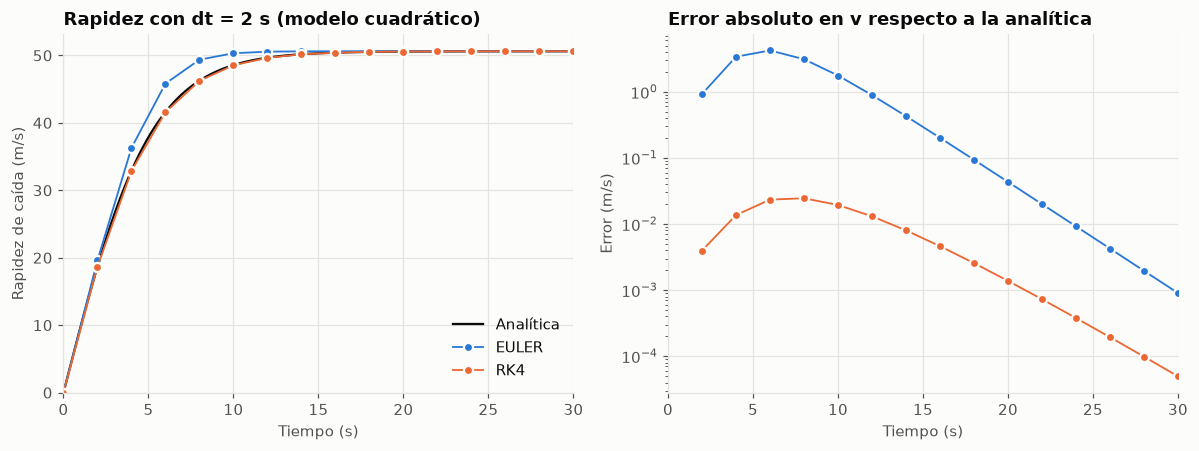
\includegraphics[width=\textwidth]{metodos_dt_grande.png}
  \caption{Izquierda: rapidez de caída del paracaidista (modelo cuadrático) con $\Delta t = \qty{2}{s}$ según la solución analítica, Euler y RK4. Derecha: error absoluto en $v$ respecto a la solución analítica, en escala logarítmica.}
  \label{fig:dt-grande}
\end{figure}

% ===========================================================================
\section{Conclusiones}
% ===========================================================================

\begin{enumerate}
  \item La resistencia del aire cambia cualitativamente la caída: en lugar de acelerar sin límite, el cuerpo tiende a una velocidad terminal $\vt$. Para el paracaidista, esto reduce la rapidez de impacto de \qty{280}{m/s} a \qty{51}{m/s}.
  \item La forma de la ley de arrastre importa aunque la velocidad terminal sea la misma: el modelo cuadrático alcanza el régimen terminal un \qty{39}{\percent} antes que el lineal (\qty{9.5}{s} contra \qty{15.5}{s}).
  \item Para objetos macroscópicos en aire el modelo adecuado es el cuadrático: en todos los casos estudiados $Re$ está entre $10^4$ y $10^7$. El modelo lineal solo es aplicable a partículas microscópicas.
  \item La influencia del aire depende de la relación entre masa y área ($\vt = \sqrt{mg/k}$), no de la masa sola. En \qty{56}{m}, la bola de boliche se comporta casi como en el vacío (\qty{1.4}{\percent} de retraso), mientras que la de ping-pong tarda más del doble.
  \item Euler y RK4 convergen con sus órdenes teóricos (1 y 4; medidos 1.00 y 4.0). RK4 es la mejor opción para este problema: con $\Delta t = \qty{0.01}{s}$ prácticamente alcanza el límite de precisión de la máquina, mientras que Euler necesitaría pasos impracticablemente pequeños para igualarlo.
  \item Reducir el paso de tiempo no siempre mejora el resultado: por debajo de cierto valor domina el error de redondeo.
\end{enumerate}

% ===========================================================================
\section{Limitaciones y sugerencias de trabajo futuro}
% ===========================================================================

El modelo utilizado hace varias simplificaciones que abren posibles extensiones:
\begin{itemize}
  \item \textbf{Densidad del aire constante.} A \qty{4000}{m} la densidad del aire es cerca de un \qty{30}{\percent} menor que a nivel del mar, por lo que la velocidad terminal real al inicio del salto es mayor. Una extensión natural es usar una atmósfera exponencial o el modelo de atmósfera estándar internacional (ISA) para obtener $\rho(y)$. Esto es imprescindible para saltos estratosféricos, como el de Felix Baumgartner en 2012, que superó la velocidad del sonido.
  \item \textbf{Coeficiente de arrastre constante.} En realidad $C_d$ depende de $Re$ (por ejemplo, la crisis de arrastre en esferas) y de la postura del paracaidista. Se podría usar una correlación empírica $C_d(Re)$.
  \item \textbf{Sin apertura del paracaídas.} Se podría cambiar $C_d A$ al alcanzar una altura dada y estudiar la transición entre dos velocidades terminales.
  \item \textbf{Movimiento solo vertical.} Una extensión a dos dimensiones (salto desde un avión en movimiento o con viento lateral) mostraría cómo el arrastre acopla las componentes horizontal y vertical.
  \item \textbf{Sin viento ni efectos de rotación}, como el efecto Magnus en pelotas que giran.
  \item \textbf{Métodos de paso fijo.} Se podría implementar un método adaptativo (por ejemplo, RK45) y una detección de eventos más precisa que la interpolación lineal.
\end{itemize}


% ===========================================================================
\begin{thebibliography}{9}
% ===========================================================================

\bibitem{burden}
R.~L. Burden y J.~D. Faires, \emph{Numerical Analysis}, 9.\textsuperscript{a} ed. Boston: Brooks/Cole, 2011.

\bibitem{taylor}
J.~R. Taylor, \emph{Classical Mechanics}. Sausalito: University Science Books, 2005.

\bibitem{white}
F.~M. White, \emph{Fluid Mechanics}, 7.\textsuperscript{a} ed. Nueva York: McGraw-Hill, 2011.

\end{thebibliography}

% ===========================================================================
\appendix
% ===========================================================================
% Apéndices (Parte 2): tablas de convergencia y reproducción.
% Se incluye desde informe.tex después de \appendix; no compilar este archivo solo.

\section{Tablas completas de convergencia}
\label{app:tablas}
% ===========================================================================

Errores absolutos máximos en el intervalo $[0, 20]$~s contra la solución analítica. La columna $p$ es el orden local calculado con el error en $v$; no se reporta cuando el error está por debajo de $10^{-9}$, donde domina el redondeo.

\begin{table}[H]
  \centering
  \small
  \caption{Convergencia del modelo lineal.}
  \label{tab:conv-lineal}
  \begin{tabular}{@{}lllclll@{}}
    \toprule
    & \multicolumn{3}{c}{Euler} & \multicolumn{3}{c}{RK4} \\
    \cmidrule(lr){2-4} \cmidrule(l){5-7}
    $\Delta t$ (s) & $e_y$ (m) & $e_v$ (m/s) & $p$ & $e_y$ (m) & $e_v$ (m/s) & $p$ \\
    \midrule
    1       & 10.157       & 1.968        & ---   & \num{1.327e-3} & \num{2.572e-4} & --- \\
    0.5     & 4.855        & 0.9408       & 1.065 & \num{7.649e-5} & \num{1.482e-5} & 4.117 \\
    0.25    & 2.376        & 0.4604       & 1.031 & \num{4.593e-6} & \num{8.901e-7} & 4.058 \\
    0.1     & 0.9387       & 0.1819       & 1.013 & \num{1.148e-7} & \num{2.224e-8} & 4.026 \\
    0.05    & 0.4675       & 0.09059      & 1.006 & \num{7.114e-9} & \num{1.379e-9} & 4.012 \\
    0.025   & 0.2333       & 0.0452       & 1.003 & \num{4.425e-10} & \num{8.585e-11} & --- \\
    0.01    & 0.09319      & 0.01806      & 1.001 & \num{1.046e-11} & \num{2.178e-12} & --- \\
    0.005   & 0.04658      & 0.009026     & 1.001 & \num{1.137e-11} & \num{2.132e-13} & --- \\
    0.0025  & 0.02328      & 0.004512     & 1.000 & \num{3.001e-11} & \num{1.421e-13} & --- \\
    0.001   & 0.009312     & 0.001805     & 1.000 & \num{1.819e-11} & \num{1.918e-13} & --- \\
    0.0005  & 0.004656     & 0.0009023    & 1.000 & \num{5.957e-11} & \num{2.416e-13} & --- \\
    0.00025 & 0.002328     & 0.0004511    & 1.000 & \num{2.046e-11} & \num{3.766e-13} & --- \\
    0.0001  & 0.0009312    & 0.0001804    & 1.000 & \num{5.366e-11} & \num{5.400e-13} & --- \\
    \bottomrule
  \end{tabular}
\end{table}

\begin{table}[H]
  \centering
  \small
  \caption{Convergencia del modelo cuadrático.}
  \label{tab:conv-cuadratico}
  \begin{tabular}{@{}lllclll@{}}
    \toprule
    & \multicolumn{3}{c}{Euler} & \multicolumn{3}{c}{RK4} \\
    \cmidrule(lr){2-4} \cmidrule(l){5-7}
    $\Delta t$ (s) & $e_y$ (m) & $e_v$ (m/s) & $p$ & $e_y$ (m) & $e_v$ (m/s) & $p$ \\
    \midrule
    1       & 16.020       & 1.920        & ---   & \num{4.150e-3} & \num{1.273e-3} & --- \\
    0.5     & 7.680        & 0.9324       & 1.042 & \num{2.621e-4} & \num{7.187e-5} & 4.146 \\
    0.25    & 3.753        & 0.4583       & 1.025 & \num{1.649e-5} & \num{4.280e-6} & 4.070 \\
    0.1     & 1.481        & 0.1816       & 1.010 & \num{4.239e-7} & \num{1.065e-7} & 4.032 \\
    0.05    & 0.7373       & 0.09051      & 1.005 & \num{2.653e-8} & \num{6.590e-9} & 4.014 \\
    0.025   & 0.3678       & 0.04518      & 1.002 & \num{1.656e-9} & \num{4.099e-10} & --- \\
    0.01    & 0.1469       & 0.01806      & 1.001 & \num{4.047e-11} & \num{1.045e-11} & --- \\
    0.005   & 0.07343      & 0.009025     & 1.000 & \num{7.731e-12} & \num{6.324e-13} & --- \\
    0.0025  & 0.03671      & 0.004512     & 1.000 & \num{1.319e-11} & \num{1.350e-13} & --- \\
    0.001   & 0.01468      & 0.001805     & 1.000 & \num{1.273e-11} & \num{2.629e-13} & --- \\
    0.0005  & 0.00734      & 0.0009023    & 1.000 & \num{3.865e-11} & \num{2.274e-13} & --- \\
    0.00025 & 0.00367      & 0.0004511    & 1.000 & \num{3.593e-11} & \num{4.761e-13} & --- \\
    0.0001  & 0.001468     & 0.0001804    & 1.000 & \num{6.776e-11} & \num{5.613e-13} & --- \\
    \bottomrule
  \end{tabular}
\end{table}

% ===========================================================================
\section{Reproducción de los resultados}
% ===========================================================================

El código se ejecuta con Python~3 y las dependencias de \texttt{requirements.txt} (\texttt{numpy}, \texttt{matplotlib} y \texttt{pillow}). Desde la raíz del repositorio:

\begin{lstlisting}[language=bash]
python -m venv .venv
pip install -r requirements.txt
python -m freefall paracaidista
python -m freefall pelotas
python -m freefall convergencia
\end{lstlisting}

Cada comando imprime una tabla de métricas y guarda sus figuras en la carpeta \texttt{results/}. Algunas opciones útiles son \texttt{--metodo euler} para usar Euler en los escenarios, \texttt{--dt} para cambiar el paso de tiempo y \texttt{--altura} para cambiar la altura inicial.


\end{document}
